\chapter{Server-Side Approaches: Development of a Gameplay
Analytics Pipeline for Suspicion Scoring}
\label{chap:three}

\epigraph{\itshape We can't solve today's problems with the mentality that created them.}{-- Albert EINSTEIN}

\stopcontents[chapters]
\startcontents[chapters]

\printMyMinitoc

\fancyhead[LE]{\textsc{\chaptername~\thechapter}}

\section{Pipeline Implementation}
\label{sec:three:one}

PROGRESSION :

La pipeline est fonctionnelle, mon problème se situe pour le moment du côté de rendre la simulation des profils aussi réaliste que possible, puisqu'il n'est pas envisageable de parser les démos du jeu pour obtenir des données réelles (ça demanderait quelques années et une équipe de développeurs payés).

Pour le moment, les profils sont encore trop "parfaits" et ne reflètent pas la réalité des joueurs humains. Il faut que je trouve un moyen de générer des profils plus diverses, qui permettront de mettre en avant l'intérêt de la notion des LSTM pour détecter les comportements anormaux sur le long terme (et donc séparer les experts des cheaters).

Les modifications que je suis en train d'apporter se situent dans la création des profils de joueurs et dans la manière dont ils sont évalués par la pipeline pour mettre en avant des résultats plus proches de ce que l'on peut observer dans la réalité et de ce qu'on peut trouver dans les sources de données externes (voir annexe 5).

L'objectif final est de séparer les casuals des experts et des cheaters, et de pouvoir détecter les comportements anormaux sur le long terme pour amener ces profils à une revue manuelle de joueurs expérimentés qui sauront faire la distinction grâce à leur expérience.
Les résultats graphiques que j'obtiens pour le moment sont les suivants :

\begin{figure}[H]
    \begin{center}
        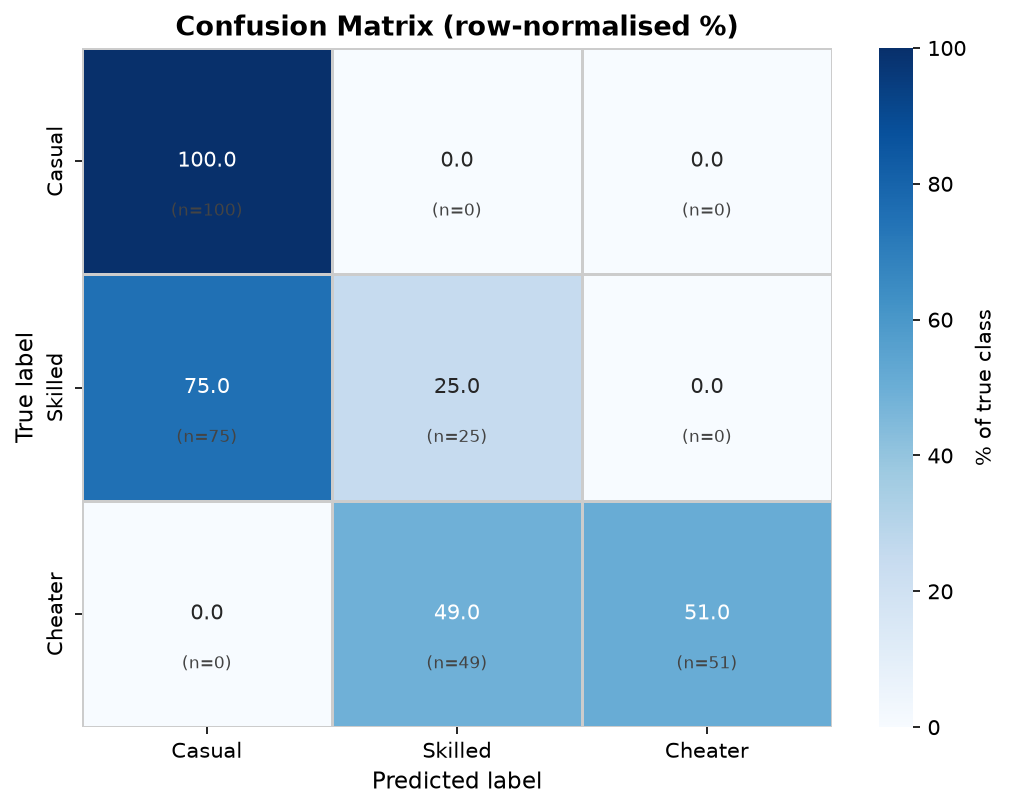
\includegraphics[height=9cm]{../images/chap03/confusion_matrix.png}
    \end{center}
    \caption{Confusion Matrix for Suspicion Scoring. Montre que l'algo de scoring n'arrive pas à différencier les profils de joueurs casual et expert. Il n'arrive pas également à différencier les profils de joueurs expert et cheater. Il est donc nécessaire de générer des profils plus réalistes pour que l'algo puisse apprendre à différencier les différents types de joueurs.}
    \label{fig:confusion_matrix}
\end{figure}

\begin{figure}[H]
    \begin{center}
        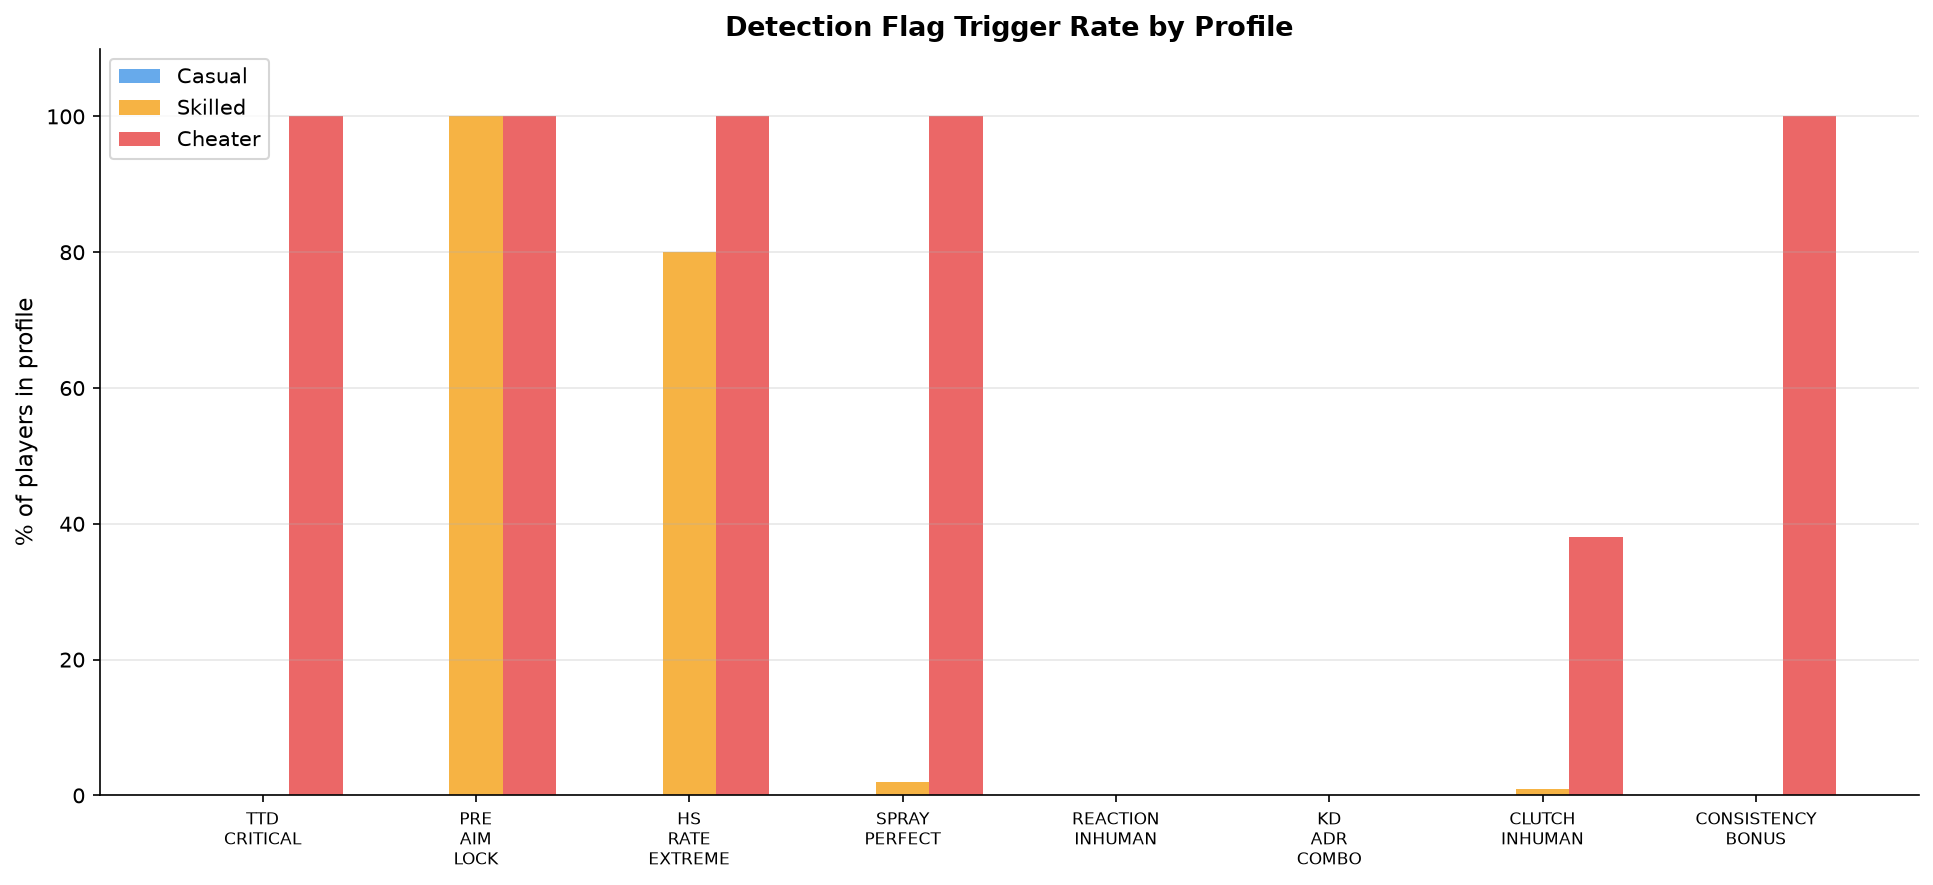
\includegraphics[height=7cm]{../images/chap03/flag_frequency.png}
    \end{center}
    \caption{Flag Frequency Distribution. Montre que l'algo de flagging se déclenche trop souvent pour les cheaters et pas assez pour les expert et les casuals. Je dois donc ajuster les seuils de déclenchement des flags pour avoir une représentation plus équilibrée et réaliste.}
    \label{fig:flag_frequency}
\end{figure}

\begin{figure}[H]
    \begin{center}
        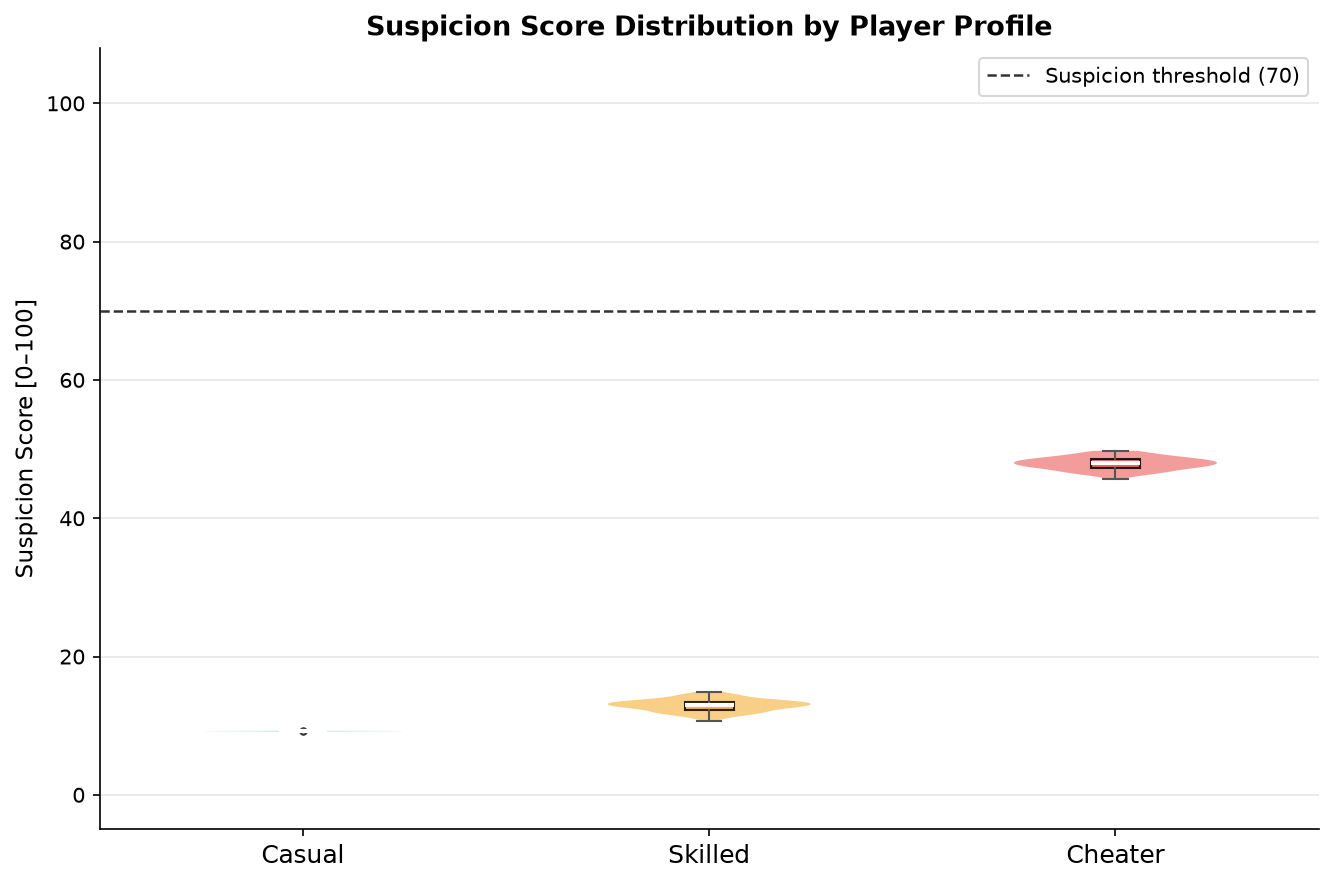
\includegraphics[height=9cm]{../images/chap03/score_distribution.png}
    \end{center}
    \caption{Score Distribution. Montre la distribution des scores attribués par l'algo de scoring. Le résultat est relativement satisfaisant pour le moment mais les scores sont globalement trop bas pour les experts et cheaters, donc les stats vont en moyenne être plus suspectes que le résultat actuel.}
    \label{fig:score_distribution}
\end{figure}

La repo est publique sur GitHub : \url{https://github.com/selligre/episen-ing3-thesis-ac-server}

\subsection{Ingestion and Scoring Objectives}
\label{sec:three:one:one}

\begin{itemize}
\item Automating telemetry-driven suspicion scoring
\item Prioritization matrix for human review (\gls{Overwatch}-style triage)
\end{itemize}

\subsection{Algorithmic Architecture and Core Concepts}
\label{sec:three:one:two}

\begin{itemize}
\item Rule-Based Foundations: Establishing game engine limits, behavioral baselines, and mechanical consistency boundaries
\item Hybrid Modeling Framework: Combining a classical deterministic heuristic algorithm (live run execution) with sequential Machine Learning concepts (Long Short-Term Memory - LSTM)
\item Flag Weighting and Temporal Aggregation: Make individual mechanical anomalies accumulate into a player history score
\end{itemize}

\subsection{Practical System Deployment}
\label{sec:three:one:three}

\begin{itemize}
\item Architecture of the analytics pipeline: https://github.com/selligre/thesis-cs2-ac-server (could use https://github.com/pnxenopoulos/awpy to help parsing data from demos)
\item Event-driven design: Comparison of real-time telemetry parsing vs. asynchronous post-match processing
\end{itemize}

\section{Dataset and Features}
\label{sec:three:two}

\subsection{Telemetry Data Model}
\label{sec:three:two:one}

\begin{itemize}
\item Aim Vectors: \gls{TTD} (TTD), pre-aim delta, and spray pattern deviation
\item Spatial and Positional Features: Cross-match positioning consistency, Opening Duels context, and Trading Efficiency windows
\item Tactical and Utility Metrics: Grenade/\gls{HE} efficiency (Average HE damage), Clutch performance variance, and overall Kill/Death ratio
\item Social/Contextual Context: Premade lobby (Party) dependencies and cross-match behavioral
\end{itemize}

\subsection{Data Sources and Profiling}
\label{sec:three:two:two}

\begin{itemize}
\item Synthetic telemetry generation: Simulating legitimate player profiles (varying from casual to highly-skilled) vs. simulated cheat profiles (aimbots, triggerbots, wallhacks and scripts)
\end{itemize}

\subsection{Data Constraints and Limitations}
\label{sec:three:two:three}

\begin{itemize}
\item Limits of server-side logs
\item Tick-rate limitations
\end{itemize}

\section{Benchmark Execution and Raw Outputs}
\label{sec:three:three}

\subsection{Experimental Protocol}
\label{sec:three:three:one}

\begin{itemize}
\item Setup of the controlled benchmarking environment
\item Execution sequence: Batch processing of simulated profiles through the classical algorithm and the LSTM layer
\end{itemize}

\subsection{Raw Evaluation Results}
\label{sec:three:three:two}

\begin{itemize}
\item Raw statistical outputs, distribution of suspicion scores and first results
\end{itemize}

\section{Analysis and Performance Discussion}
\label{sec:three:four}

\subsection{Net Detection Results}
\label{sec:three:four:one}

\begin{itemize}
\item Link between extreme data profiles and cheaters
\item Robustness assessment: Evaluating the accuracy when mixing in high-skill profiles
\end{itemize}

\subsection{Mitigating the High-Skill Bias}
\label{sec:three:four:two}

\begin{itemize}
\item Analyzing the conceptual limits of false positives
\item Differentiating anomalous expert playstyles (exotic but legitimate behaviors) from software-assisted mechanics
\item Comparative Analysis: Contrasting our suspicion-scoring pipeline with commercial performance platforms like \gls{Leetify.gg} (How metrics designed for coaching can be repurposed for anti-cheat signaling)
\end{itemize}

\subsection{Future Optimizations}
\label{sec:three:four:three}

\begin{itemize}
\item Build accurate data profiles faster
\item Take into account external factors (number of cheaters in their friends list, age of the account, number of hours played related to the skill-level shown… things that experimented players learn to recognize but that the software fails to implement)
\end{itemize}

\section{Comparison with Kernel-level approach}
\label{sec:three:five}

This capability gap is directly acknowledged in the literature: open-source behavioural detection trained exclusively on server-side kill telemetry has been shown to identify players subsequently confirmed as cheating via VAC ban, suggesting that hardware-level cheats — which leave no software footprint detectable by a kernel driver — nonetheless produce statistically anomalous gameplay signatures exploitable from the server \cite{Loo2025}.

\begin{itemize}
\item Effectiveness
\item Intrusiveness
\item Implications for the FPS / esport industry
\item Player perception
\item Human validation
\end{itemize}
